\chapter{相关工作}

\section{战术数据链(Tactical Data Link)}
战术数据链(Tactical Data Link, TDL)是实现作战平台、传感器与指挥控制中心之间实时数据传输与信息共享的核心通信方式\cite{AFMAN_13_116_Vol1_2020,EverythingRF_Link16_Band}。  
自20世纪70年代起,随着 {JTIDS} 与 {Link16} 的逐步形成,战术数据链体系不断发展,已成为现代联合作战的重要基础设施\cite{DLS_MIDS_JTRS_2021,BAE_Link16_Terminals_2025}。

战术数据链的发展历程可以追溯到冷战时期,当时美军迫切需要一种能够在复杂电磁环境下实现多平台协同作战的通信手段。早期的战术数据链主要基于模拟信号传输,如Link 4A和Link 11,这些系统虽然在一定程度上满足了当时的作战需求,但在抗干扰能力、数据传输速率和网络容量方面存在明显不足。随着数字通信技术的快速发展,以Link 16为代表的数字战术数据链应运而生,标志着战术数据链技术进入了新的发展阶段。

现代战术数据链的核心特征包括:实时性、可靠性、安全性和互操作性。实时性要求系统能够在毫秒级时间内完成关键信息的传输和处理,这对于时间敏感的作战任务至关重要。可靠性体现在系统能够在恶劣的电磁环境和复杂的战场条件下保持稳定的通信连接。安全性则通过先进的加密算法和抗干扰技术来保障,确保敏感信息不被敌方截获或干扰。互操作性使得不同国家和不同军种之间的平台能够实现信息共享和协同作战,这是现代联合作战的基本要求。

在技术架构方面,战术数据链通常采用分层设计,包括物理层、数据链路层、网络层和应用层。物理层负责信号的调制解调和传输,数据链路层处理帧同步、错误检测和流量控制,网络层管理路由选择和网络拓扑,应用层则提供具体的业务功能。这种分层架构不仅提高了系统的可维护性和可扩展性,还为不同厂商的设备互操作提供了标准化的接口。

随着网络中心战概念的提出和信息化战争的发展,战术数据链的作用范围不断扩大,从最初的单一平台间通信发展为支持整个作战体系的网络化通信基础设施。现代战术数据链不仅要支持传统的语音和数据传输,还要承载视频、图像、态势信息等多种类型的数据,这对系统的带宽和处理能力提出了更高的要求。  

战术数据链技术经历了多个发展阶段,从早期的Link 4A到现代的Link 16,每种数据链都有其特定的技术特点和适用场景。为了全面了解不同战术数据链的性能差异,表\ref{table_tdl_compare}详细对比了典型战术数据链的关键技术参数,包括传输速率、抗干扰能力、覆盖范围和应用场景等核心指标。通过对比分析可以看出,Link 16在传输速率、抗干扰能力和覆盖范围方面都具有显著优势,这也是其成为现代战术数据链主流标准的重要原因。

\begin{table}[!htb]
    \caption{典型战术数据链对比}
    \label{table_tdl_compare}
    \centering
    \adjustbox{width=0.8\textwidth,center}{%
    \begin{tabular}{lcccc}
        \hline
        \textbf{数据链类型} & \textbf{速率(kbps)} & \textbf{抗干扰} & \textbf{覆盖范围} & \textbf{典型应用} \\
        \hline
        Link 11 & 1.8--2.25 & 较弱 & 约 300 km & 早期空海通信 \\
        Link 16 & 31.6--115.2 & 强 & 约 500 km & 联合作战、火力协调 \\
        Link 22 & 2.4--275 & 强 & 超视距(BLOS) & NATO 联盟协同 \\
        \hline
    \end{tabular}%
    }
\end{table}

如图\ref{fig_tdl_architecture} 所示,战术数据链通过多平台互联形成统一网络,实现了态势共享和联合打击。

\begin{figure}[!htb]
    \centering
    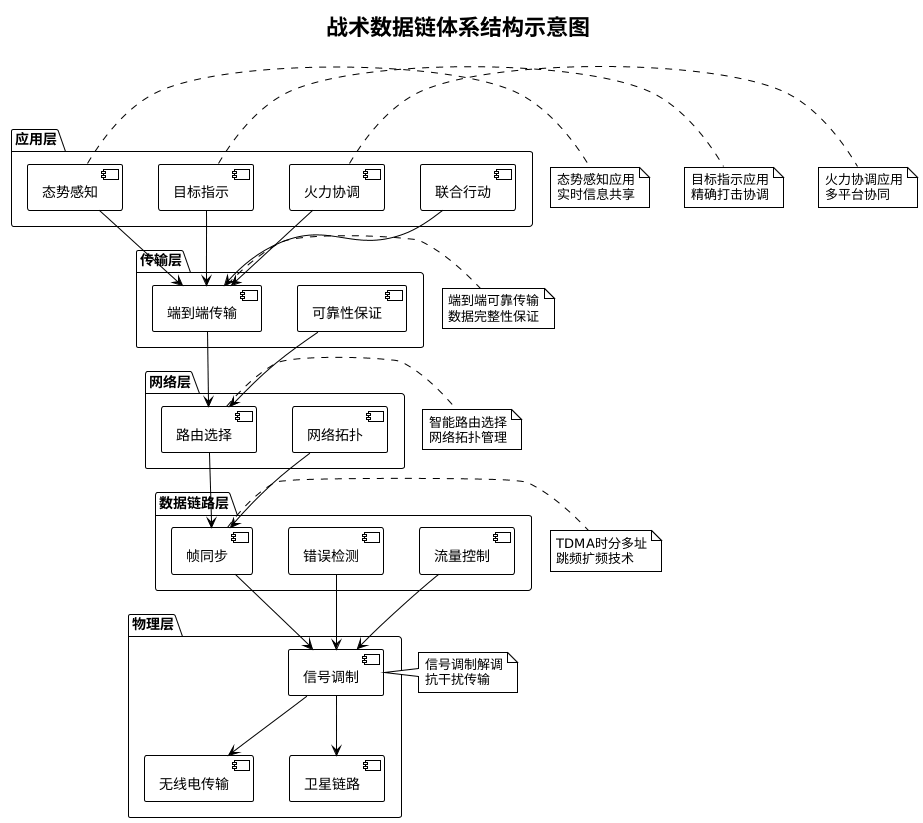
\includegraphics[width=0.8\textwidth,height=0.5\textheight,keepaspectratio]{chapters/fig-0/tdl_architecture_simple.png}
    \caption{战术数据链体系结构示意图}
    \label{fig_tdl_architecture}
\end{figure}

在北约和美军体系中,{Link16} 以其高速率、抗干扰和加密能力被广泛应用于空、海、地等平台\cite{Ultra_ADSI_2023}。其典型应用包括态势感知、目标指示、火力协调和联合行动等方面。然而,随着多链并行与跨域作战需求的增加,传统链路逐渐暴露出互操作性不足和资源利用率低的问题。

Link 16的技术优势主要体现在其采用的时分多址(TDMA)接入方式和跳频扩频技术。TDMA技术通过时间片分配的方式,使得多个平台能够在同一频段上同时工作而不会相互干扰,这大大提高了频谱利用效率。跳频扩频技术则通过快速改变载波频率来对抗敌方的干扰和截获,增强了系统的抗干扰能力和安全性。此外,Link 16还采用了先进的加密算法,如KGV-8加密机,确保传输信息的安全性。

在应用层面,Link 16支持多种类型的J系列消息,包括J2.0(初始入网)、J3.0(航迹管理)、J3.2(空中航迹)、J3.3(水面航迹)、J3.5(空中航迹扩展)、J7.0(任务管理)、J12.0(电子战)等。这些消息类型覆盖了现代作战的各个方面,从基本的航迹信息到复杂的任务协调,为多平台协同作战提供了完整的信息支撑。

然而,随着作战环境的复杂化和作战需求的多样化,Link 16也面临着一些挑战。首先是带宽限制问题,虽然Link 16的数据传输速率相比早期系统有了显著提升,但在处理大量高分辨率图像、视频等多媒体数据时仍显不足。其次是互操作性问题,不同国家和不同厂商的设备在实现Link 16标准时可能存在细微差异,这影响了系统的互操作性。最后是网络安全问题,随着网络攻击技术的不断发展,传统的加密和认证机制可能面临新的威胁。

为了解决这些问题,各国军方和工业界正在积极研发新一代战术数据链技术。这些新技术在保持Link 16核心优势的基础上,重点提升了带宽容量、增强了网络安全防护能力,并改善了与现有系统的兼容性。同时,人工智能、机器学习等新兴技术的引入,也为战术数据链的智能化发展提供了新的机遇。

\section{MIL-STD-6016 标准框架与特点}
MIL-STD-6016 作为 {Link16} 的核心标准,对 J 系列报文的格式、语义及应用场景做出了详细规定\cite{ASSIST_6016_2024,CJCSM_6235_01_2025}。其主要特点包括:  

(1)统一的 J 系列消息目录,覆盖作战控制、目标指示与火力支援等功能;  

(2)采用时分多址(TDMA)机制,保证在高密度网络中的有序通信;  

(3)抗干扰能力强,结合跳频扩频和加密算法,提升系统的安全性和鲁棒性;  

(4)具备扩展性,可通过 {JREAP} 协议实现超视距(BLOS)传输,并与 {TTNT} 等新型战术网络互操作。

此外,MIL-STD-6020 明确了跨数据链数据转发与映射的规则;NATO 的 STANAG 5602 及其配套 SIMPLE 规范为异构链路互连提供了标准化接口;而 SISO 标准给出了 {Link16} 仿真的数据模型与交互定义\cite{Ultra_MDLMS_2021}。这些标准共同构成了战术数据链互操作的规范框架。

MIL-STD-6016标准的制定过程体现了美军在战术数据链标准化方面的长期努力。该标准不仅详细规定了J系列消息的格式和语义,还建立了完整的消息处理流程和错误处理机制。标准中的每个消息类型都有明确的定义,包括消息结构、字段含义、取值范围、处理规则等,这为不同厂商的设备实现提供了统一的规范。

图\ref{fig_j_series_message_structure}展示了MIL-STD-6016标准中J系列消息的完整结构体系,清晰呈现了消息的分类和组织方式。该图按照功能将J系列消息分为六大类:作战控制类(J0-J9)、电子战类(J10-J19)、情报类(J20-J29)和武器协调类(J30-J39),每类消息都有其特定的应用场景和功能定位,体现了标准设计的系统性和完整性。

\begin{figure}[H]
    \centering
    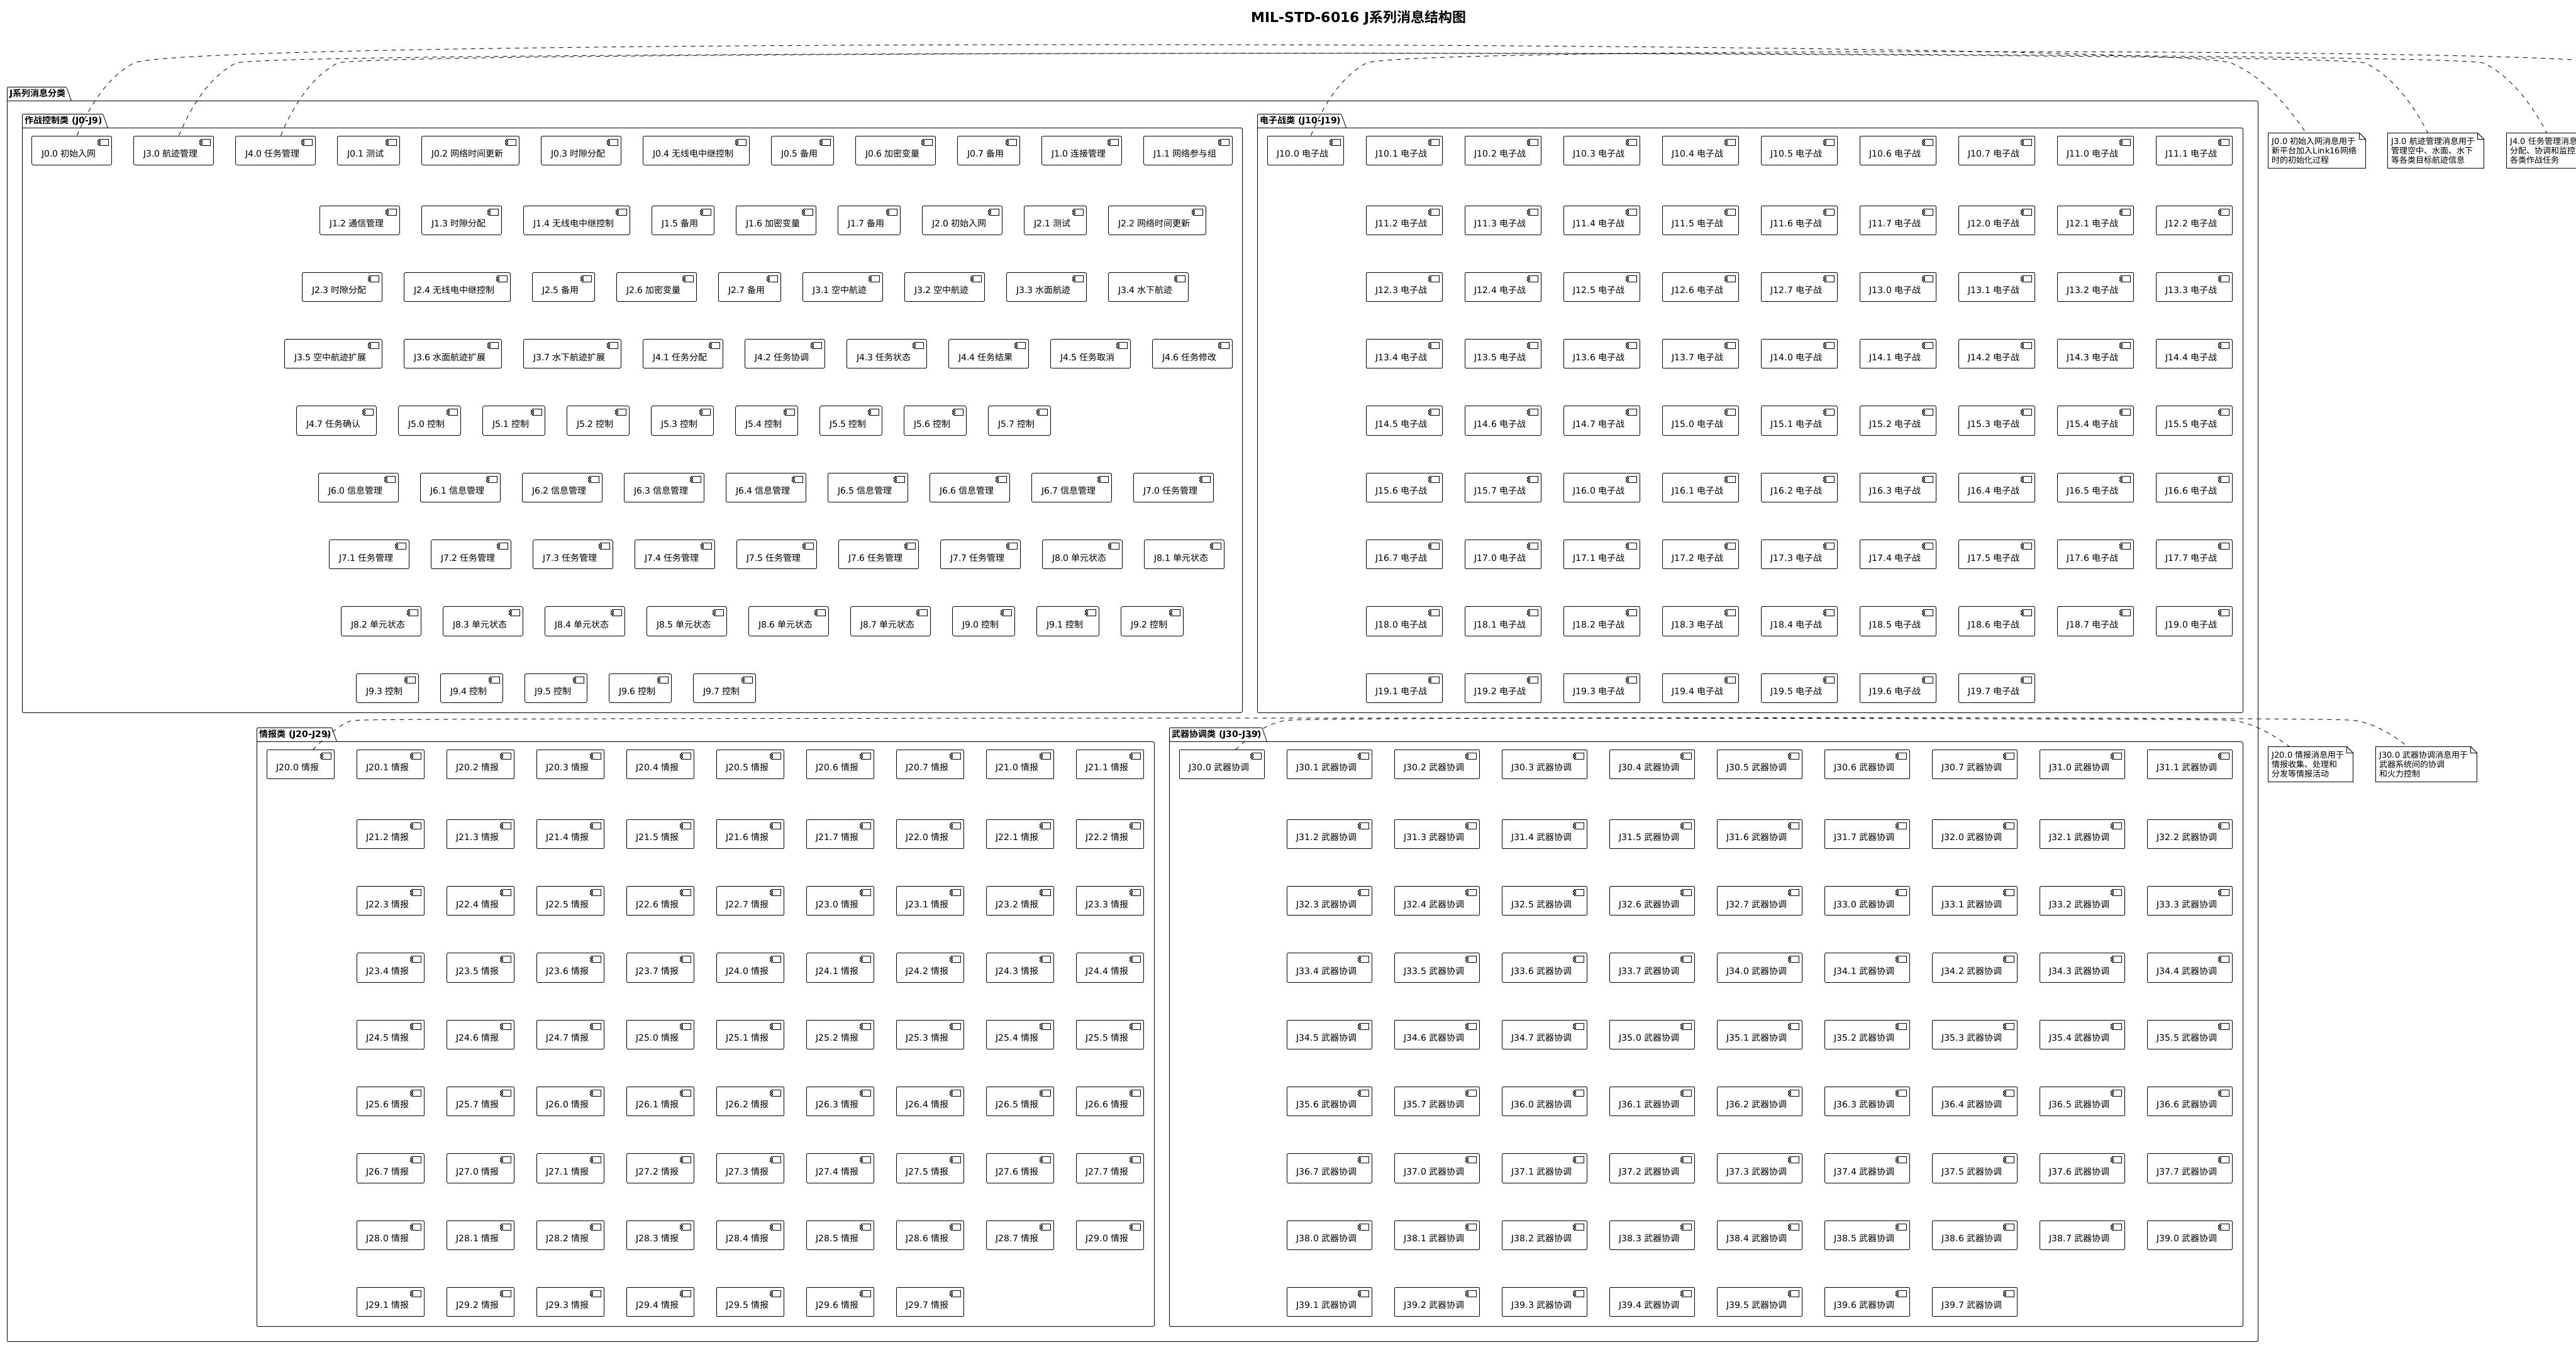
\includegraphics[width=0.85\textwidth,height=0.6\textheight,keepaspectratio]{chapters/fig-0/j_series_message_structure.png}
    \caption{MIL-STD-6016 J系列消息结构图}
    \label{fig_j_series_message_structure}
\end{figure}

在消息格式方面,MIL-STD-6016采用了固定长度和可变长度相结合的设计。固定长度消息具有处理简单、传输效率高的优点,适用于对实时性要求较高的应用场景。可变长度消息则能够适应不同复杂度的信息传输需求,提高了系统的灵活性。这种设计使得Link 16能够同时支持简单的状态报告和复杂的任务协调信息。

标准还特别关注了消息的语义一致性问题。由于战术数据链涉及多个军种和多个国家的平台,确保消息语义的一致性对于实现真正的互操作至关重要。MIL-STD-6016通过建立详细的数据字典和语义规范,为不同平台之间的信息交换提供了统一的理解基础。

随着技术的不断发展,MIL-STD-6016标准也在持续更新和完善。新版本的标准不仅增加了新的消息类型,还改进了现有的消息格式,以适应新的作战需求和技术发展。同时,标准还加强了对网络安全和抗干扰能力的要求,体现了现代战争对通信系统安全性的重视。

在标准实施方面,各国军方和工业界都投入了大量资源来确保设备的标准化和互操作性。这包括建立标准化的测试流程、认证机制和兼容性验证程序。通过这些措施,MIL-STD-6016标准得以在全球范围内得到有效实施,为多国联合作战提供了重要的技术支撑。

表\ref{table_mil_std_comparison}对比分析了MIL-STD-6016与其他相关标准的特点、应用范围和互操作性能力。从表中可以看出,MIL-STD-6016作为Link16的核心标准,在消息格式、传输机制和互操作性方面都具有显著优势,为战术数据链的标准化和互操作提供了重要的技术基础。

\begin{table}[!htb]
    \caption{MIL-STD-6016相关标准对比分析表}
    \label{table_mil_std_comparison}
    \centering
    \adjustbox{width=0.95\textwidth,center}{%
    \begin{tabular}{lcccc}
        \hline
        \textbf{标准名称} & \textbf{主要功能} & \textbf{应用范围} & \textbf{互操作性} & \textbf{技术特点} \\
        \hline
        MIL-STD-6016 & J系列消息格式定义 & Link16战术数据链 & 强 & TDMA、跳频扩频、加密 \\
        & 消息语义规范 & 联合作战平台 & & 固定/可变长度消息 \\
        & 处理流程标准 & 多军种协同 & & 实时性、可靠性 \\
        \hline
        MIL-STD-6020 & 跨数据链转发 & 多链路互连 & 中等 & 数据映射、格式转换 \\
        & 数据映射规则 & 异构系统集成 & & 协议适配、路由选择 \\
        & 互操作接口 & 联盟作战 & & 标准化接口 \\
        \hline
        STANAG 5602 & NATO互操作标准 & NATO成员国 & 强 & 统一数据格式 \\
        & SIMPLE规范 & 联盟协同作战 & & 标准化接口 \\
        & 异构链路互连 & 多国联合作战 & & 兼容性保证 \\
        \hline
        SISO标准 & 仿真数据模型 & Link16仿真系统 & 中等 & 仿真接口标准 \\
        & 交互定义 & 训练与测试 & & 数据模型规范 \\
        & 仿真互操作 & 系统验证 & & 标准化仿真 \\
        \hline
    \end{tabular}%
    }
\end{table}

\section{微服务架构}

微服务架构(Microservice Architecture, MSA)作为软件工程领域的重要演进方向,其理论基础可追溯至 2010 年前后。最早由 James Lewis 与 Martin Fowler 在 2014 年系统阐述,他们认为微服务是一种以业务能力为核心的分布式架构模式,强调服务自治、松耦合与独立部署。与传统单体应用相比,微服务能够在快速迭代与持续交付中保持模块独立性,从而显著提升系统的灵活性与可维护性。自 2015 年被称为“微服务元年”以来,Netflix、Amazon、Google 等企业率先在大规模分布式系统中采用微服务架构,通过构建服务注册中心、API 网关与容错机制,实现了服务治理、动态伸缩与高可用部署,推动了这一理念从企业实践走向学术研究的深入阶段。

进入 2018–2020 年,国外学术界开始聚焦于微服务的系统化研究与性能分析。Waseem 等人基于 106 份工业问卷与多项访谈,系统总结了微服务系统的设计、监控与测试现状。他们指出领域驱动设计(DDD)与基于业务能力的服务划分已成为主流方法,API 网关与 Backend-for-Frontend 架构被广泛采用,而监控层面则以资源利用率、负载均衡与日志聚合为核心指标。研究还发现,跨服务通信复杂性、边界划分模糊与自动化测试不足是微服务工程中的主要难题 \cite{Waseem2021Design}。这一时期的研究为微服务架构的质量属性、监控机制和测试框架提供了经验基础。

伴随分布式数据系统与云原生技术的发展,数据管理成为微服务研究的重要方向。Laigner 等人在《Data Management in Microservices》中系统梳理了 30 多个工业案例与学术成果,指出“每服务独立数据库”(Database per Service)模式虽有助于解耦,但也带来了跨服务事务与数据一致性难题。他们提出在异构数据库环境下,应综合采用 Saga 模式、事件驱动与最终一致性策略以平衡性能与可靠性 \cite{Laigner2021Data}。后续研究进一步提出面向微服务的基准测试体系,如《Benchmarking Data Management Systems for Microservices》与《Online Marketplace》两篇工作,从事务处理、事件一致性与数据复制角度评估数据管理系统性能,为微服务数据库化演进提供了实验标准 \cite{BenchmarkingDataMgmt2024,OnlineMarketplace2024}。与此同时,Giamattei 等人开展了针对 71 种微服务监控工具的系统性灰文献回顾,总结出资源监控、日志追踪与可观测性平台的实践经验,揭示出当前工具生态存在指标标准不统一与跨层数据整合不足的问题 \cite{MonitoringTools2023}。

在安全与治理层面,微服务系统的复杂性引发了访问控制与认证机制的研究热潮。多项工作强调微服务的“零信任”架构思想,通过轻量级认证(OAuth2.0、JWT)与服务网格(Service Mesh)实现安全通信、流量隔离与细粒度权限控制。这些研究为后续的 DevSecOps 与自动化安全管控提供了理论与技术支持。国外学术界还开始关注微服务架构的智能演化与自适应机制,通过人工智能与机器学习方法实现服务部署优化、容器调度与异常检测的自动化,从而推动微服务从静态架构走向动态自组织系统。

在国内,微服务的理论与实践探索大约始于 2010 年前后。2007 年阿里巴巴集团在淘宝平台中引入分布式服务框架,为我国微服务化奠定了技术基础。此后,Dubbo、Spring Cloud Alibaba、ServiceComb 等国产开源框架相继出现,极大推动了微服务在企业级系统中的普及。进入 2020 年以后,国内学术界与军工科研机构开始关注微服务在复杂信息系统中的应用,探索将其引入战术通信与指挥控制平台。研究内容主要集中在服务拆分原则、容器化部署、服务编排与跨节点一致性控制等方面。一些研究单位已在态势信息处理与仿真平台中部署微服务集群,实现任务模块的自治运行与动态伸缩。总体而言,我国的研究重心正在从框架复用与工程应用向体系设计与性能验证转变,逐步形成适配于军事通信系统特性的微服务体系结构。

图\ref{fig_microservices_evolution_timeline}展示了微服务架构的发展时间线,清晰呈现了从理论基础阶段到智能化发展阶段的完整演进过程。该图从时间维度展示了国外研究从2010-2014年的概念提出和理论建立,到2015-2017年的企业实践和云原生发展,再到2018-2020年的系统化研究和2021年至今的智能化发展,以及国内从2007年的技术基础到2020年的应用探索的发展路径,体现了微服务技术的成熟度和应用深度。

\begin{figure}[H]
    \centering
    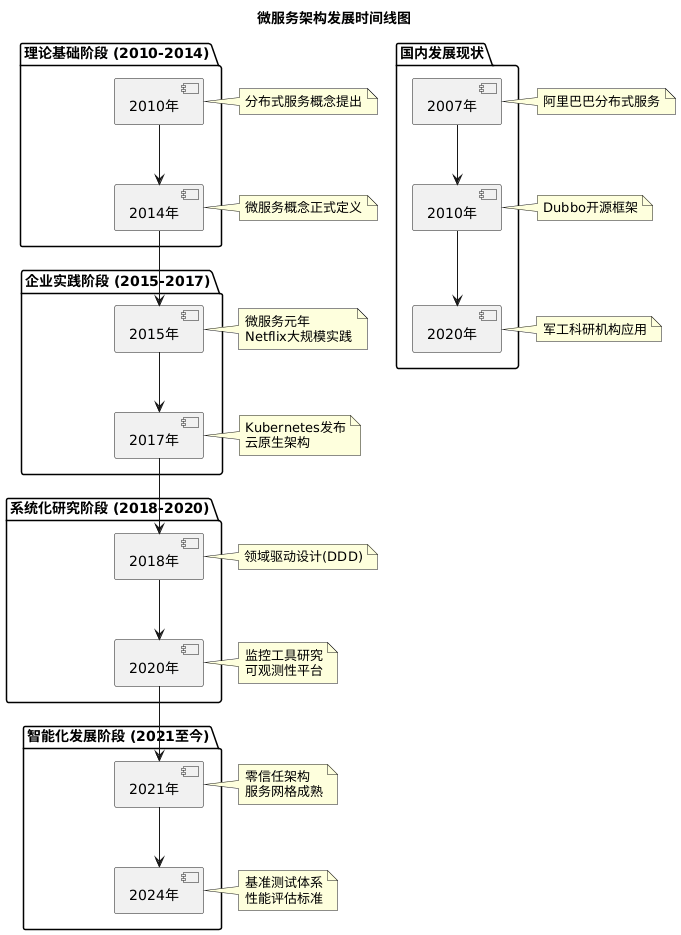
\includegraphics[width=0.8\textwidth,height=0.6\textheight,keepaspectratio]{chapters/fig-0/microservices_evolution_timeline.png}
    \caption{微服务架构发展时间线图}
    \label{fig_microservices_evolution_timeline}
\end{figure}


\section{语义互操作}

语义互操作(Semantic Interoperability)是异构系统在数据交换过程中实现“语义层理解一致”的关键能力,其核心目标是让信息在不同系统、组织或领域间传输时,不仅保持结构一致,还能被准确解释和复用。该概念最早起源于语义网与本体论研究,通过形式化语义模型描述数据背后的概念及其关系,为复杂系统间的理解一致提供理论基础。随着信息系统复杂性与数据异构性的增加,语义互操作逐渐成为人工智能、云计算、医疗健康、工业物联网等领域的核心研究方向。

在国际研究领域,早期的语义互操作工作侧重于标准体系的构建与模型分层。SISO、NATO 及 ISO 等机构提出的多层互操作模型,将信息交互划分为语法层、语义层与语用层\cite{SISO_STD_002_2006,CJCSI_6610_01F_2021},为后续研究提供了统一框架。进入 2010 年代后,学者们开始关注本体(Ontology)在语义互操作中的作用。Mishra 与 Jain 提出了“语义知识宝库”(Semantic Knowledge Treasure)概念,利用 OWL 与 SPARQL 实现异构资源的统一语义表示与查询\cite{Mishra2018Semantic}。此类研究的出现标志着语义互操作从概念层标准化向知识层融合迈进。

近年来,随着知识图谱、人工智能与自动推理技术的发展,语义互操作研究呈现出智能化与自动化的趋势。Bernasconi 等人提出“本体解包”(Ontological Unpacking)方法,对现有概念模型进行本体层剖析,以揭示模型隐含的语义结构并提升模型互操作性\cite{Bernasconi2022Ontological}。Guizzardi 与 Guarino 则在《Semantics, Ontology and Explanation》中探讨了语义互操作的解释性问题,强调应通过语义透明性与本体承诺(Ontological Commitment)提升系统间的可理解性与信任性\cite{Guizzardi2023Explanation}。此外,机器学习与规则引擎结合的语义映射算法被用于自动发现概念对应关系,实现跨领域知识的语义对齐与复用。

随着云计算和分布式系统的普及,语义互操作的研究进一步扩展到跨平台与多云环境。Hamdan 与 Admodisastro 提出一种基于本体的多云语义互操作参考架构,在架构中引入语义中枢(Semantic Hub)用于协调不同云平台的语义模型,从而实现服务间的语义一致访问\cite{Hamdan2023Reference,SemanticMultiCloud2024}。他们指出,在异构云环境中保持语义一致性需要在架构层、数据层与治理层之间建立协同机制。此外,语义互操作正与数据治理、知识集成、可解释人工智能等研究方向深度融合,为跨系统协同提供基础设施支持。

国内学术界在语义互操作领域的研究起步于 2000 年代的语义网工程,近年来伴随知识图谱与人工智能的快速发展而加速推进。研究方向包括语义本体构建、跨领域语义映射、语义检索与语义推理系统设计等。学者们提出基于知识图谱的语义关系建模框架,通过实体对齐与语义索引提升异构数据的可融合性;同时,在智慧城市、医疗、交通和工业互联网等场景中,语义互操作被用于实现多源数据的协同管理与智能决策。当前研究逐渐从"语义建模"走向"语义计算",关注语义理解、自动推理与动态本体演化的结合,以满足实时、可解释的智能系统需求。

图\ref{fig_semantic_interop_architecture}展示了语义互操作的架构层次,清晰呈现了从物理层到语用层的四层架构模式。该图详细展示了语义互操作系统的层次结构:物理层负责传输协议和网络连接,语法层处理数据格式和消息结构,语义层通过本体模型和概念映射实现语义一致性,语用层关注业务规则和上下文理解,以及互操作机制中的语义中枢、映射引擎、转换器和验证器,体现了语义互操作技术的理论深度和系统完整性。

\begin{figure}[H]
    \centering
    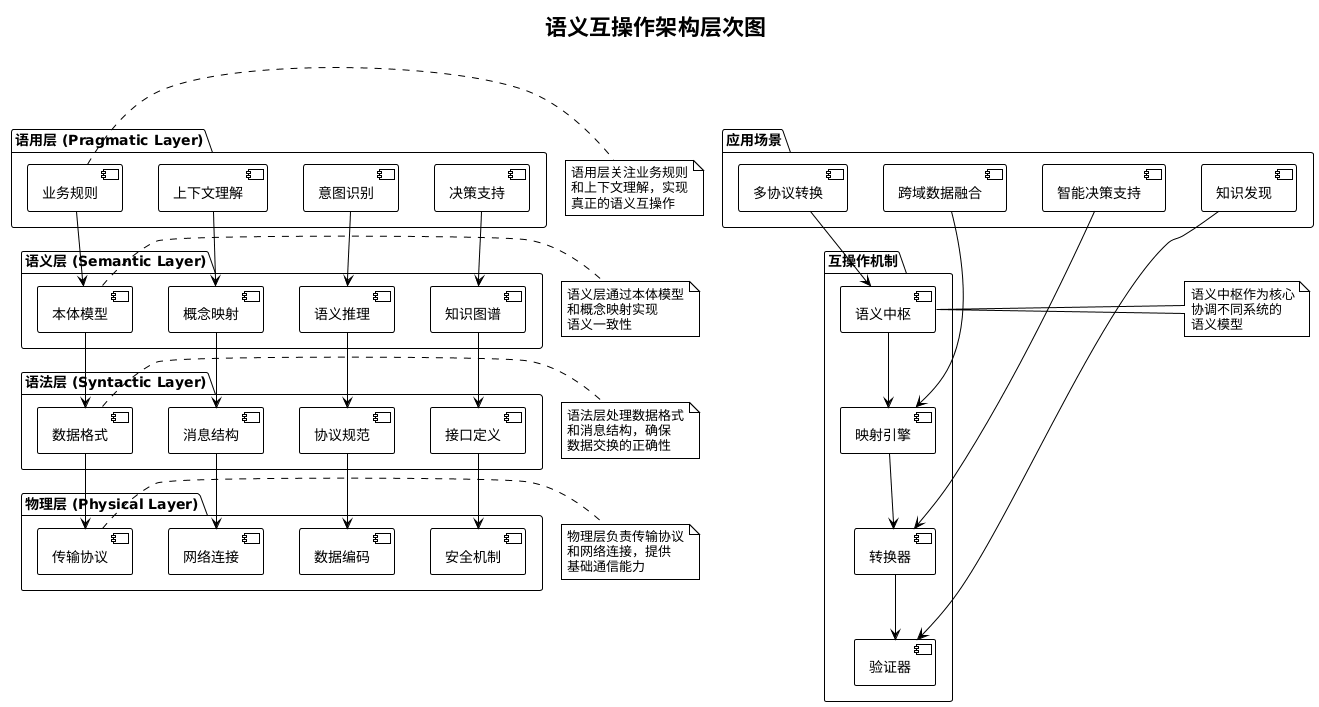
\includegraphics[width=0.85\textwidth,height=0.7\textheight,keepaspectratio]{chapters/fig-0/semantic_interop_architecture.png}
    \caption{语义互操作架构层次图}
    \label{fig_semantic_interop_architecture}
\end{figure}


\section{自动化处理}

自动化处理技术在复杂信息系统建设中具有基础性作用,其核心目标是将非结构化或半结构化文档(如 PDF、Word、XML、JSON 等)自动解析、识别并导入数据库或知识系统,以实现高效、准确的信息获取与建模。该方向的研究经历了从基于规则的文档解析到机器学习与深度学习驱动的智能化处理的演变过程,近年来在自然语言处理、文档智能(Document Intelligence)与多模态学习的推动下取得了显著进展。

早期的自动化文档处理研究以版面分析(Layout Analysis)和文本块识别为主要方法。典型工作包括基于光学字符识别(OCR)的文本抽取、表格检测与区域定位算法。这一阶段的研究主要依赖启发式规则与图像分割算法,如 PDFMiner、Apache Tika 等工具框架,通过对文本流与版面结构的分析实现基本的内容解析。然而,这些方法难以处理复杂文档中的语义结构与跨页逻辑关系。

随着深度学习和自然语言处理技术的成熟,研究重心逐步转向基于神经网络的文档理解与语义建模。2020 年以来,Google、Microsoft、Adobe 等机构相继提出了视觉语言融合模型(Vision-Language Models)用于文档解析。例如,Xu 等提出的 LayoutLM 系列模型\cite{Xu2020LayoutLM,Xu2022LayoutLMv3},通过联合建模文本、位置与视觉信息,实现了对文档结构与语义的深层理解,广泛应用于表格识别、关键信息抽取与文档分类任务。相关研究表明,基于 Transformer 的多模态模型在 PDF 结构分析中的表现显著优于传统方法,为复杂格式文档的自动化解析提供了通用方案。

在信息抽取与结构化导入方向,学者们提出了多种智能抽取与标准映射框架。Li 等在《DocParser: Document Parsing and Structured Data Import》\cite{Li2021DocParser} 中提出一种结合文本分块、实体识别与模板匹配的自动导入机制,实现 PDF 与 XML 文档的语义级结构化导入。与此同时,研究者将知识图谱构建与自动文档处理相结合,通过实体识别、关系抽取与语义对齐实现从原始文档到知识图谱的自动生成,为数据标准化与语义互操作奠定了基础。此类方法已在专利文档、医学报告与技术标准文件的自动建模中得到验证。

近年来,自动化处理逐渐向自监督学习与跨模态理解方向发展。模型不再依赖人工标注,而是通过大规模文档预训练实现通用特征学习。例如,Powalski 等提出的 DocFormer 模型\cite{Powalski2021DocFormer},采用文本与视觉双流 Transformer 结构,在文档分类与表格提取任务上达到了最优性能。进一步的研究探索将大型语言模型(LLM)与文档理解相结合,实现跨模态语义推理与任务自适应能力\cite{Wang2023DocumentLLM},标志着文档自动化处理进入“语义理解驱动”的新阶段。

国内对自动化文档处理的研究主要集中在结构化识别与智能导入系统的工程化实现方面。科研院所与企业围绕 PDF 解析、表格抽取、字段标注与标准化导入等问题展开研究,开发了基于深度学习的 OCR 引擎与语义分层系统。例如,百度文心、阿里达摩院与华为诺亚方舟实验室均提出了面向企业文档与技术标准的多模态解析方案,部分系统已在电子政务、科研档案与装备资料管理中得到应用。尽管如此,当前国内研究仍存在跨格式迁移能力弱、语义抽象层次有限、自动验证与错误纠正机制不足等问题,尚需在知识表示、语义约束与可解释性方面进行深入研究。

图\ref{fig_document_processing_evolution}展示了文档自动化处理技术的演进历程,清晰呈现了从规则驱动阶段到智能化阶段的完整发展脉络。该图从技术发展角度展示了文档处理技术的四个发展阶段:2000-2010年的规则驱动阶段主要依赖启发式算法,2010-2020年的机器学习阶段引入视觉语言融合模型,2020-2023年的深度学习阶段采用Transformer架构,2023年至今的智能化阶段实现多模态融合和自适应机制,以及在电子政务、科研档案、装备资料、技术标准等领域的应用,体现了文档自动化处理技术的成熟度和应用广度。

\begin{figure}[H]
    \centering
    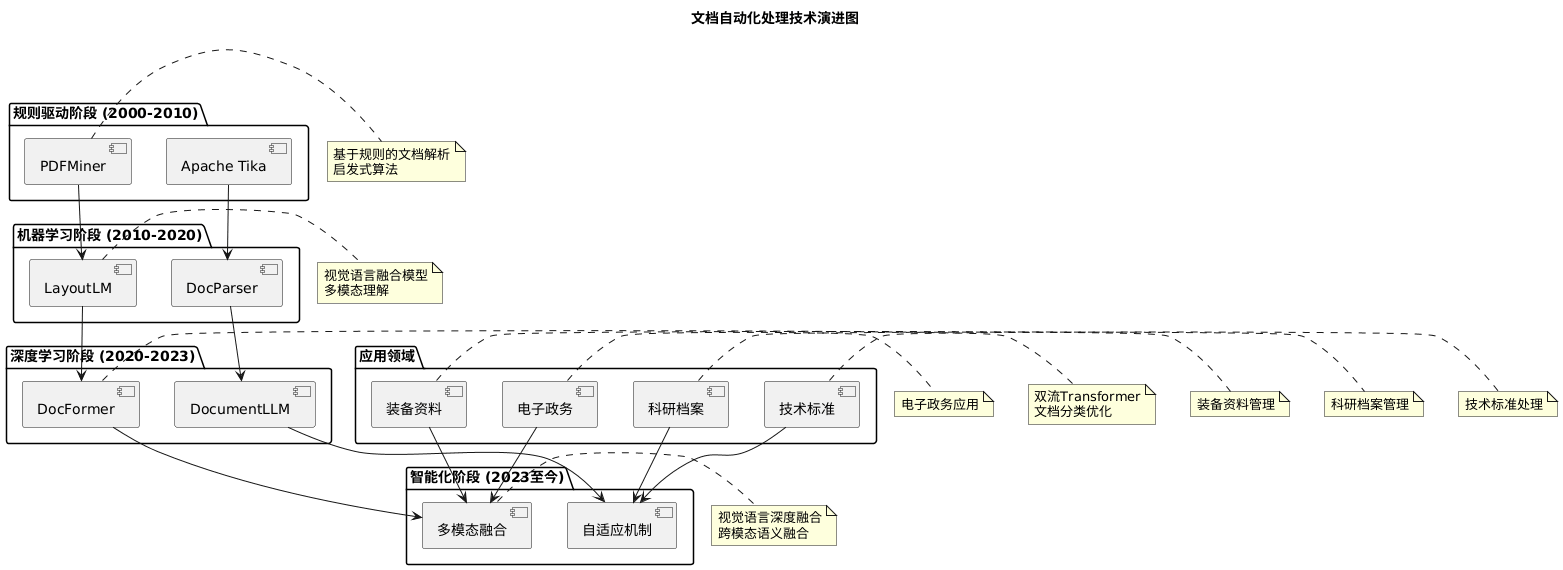
\includegraphics[width=0.8\textwidth,height=0.6\textheight,keepaspectratio]{chapters/fig-0/document_processing_evolution.png}
    \caption{文档自动化处理技术演进图}
    \label{fig_document_processing_evolution}
\end{figure}

